\documentclass{article}

\usepackage{amsmath}
\usepackage[english, russian]{babel}
\usepackage[utf8]{inputenc}
\usepackage[T2A, T1]{fontenc}
\usepackage{graphicx}

\title{Модель Кейна--Меле}
\author{Евгений Аникин}

\begin{document}
	\maketitle
	Пока что я не смог написать никаких формул для краевых состояний в этой модели (они
	получаются очень громоздкие). Но зато я нашёл уровни энергии для полосы конечной
	толщины численно. Картинка получилась такая же, как в статье.
	\section{Однородная решётка}
	Запишем гамильтониан из оригинальной статьи в менее компактном, но более удобном виде:
	\begin{multline}
		H = t\sum a_{mn}^\dagger(b_{mn} + b_{m,n-1} + b_{m+1,n-1}) + \mbox{h.c.} \\
		+it_2 \sum a_{mn}^\dagger(a_{m,n+1} + a_{m-1,n} + a_{m+1,n-1}) + \mbox{h.c.} \\
		-it_2 \sum b_{mn}^\dagger(b_{m,n+1} + b_{m-1,n} + b_{m+1,n-1}) + \mbox{h.c.} 
	\end{multline}
	Здесь имеется в виду, что проекция спина $s_z$ равна единице.
	Операторы $a$, $b$ ``сидят`` в узлах шестиугольной решётки, базис которой мы выберем так:
	\begin{equation}
		\vec{x} = \left(\begin{matrix} \frac32 \\ \frac{\sqrt{3}}{2} \end{matrix}\right), \quad
		\vec{y} = \left(\begin{matrix} 0 \\ \sqrt{3} \end{matrix}\right)
	\end{equation}
	После преобразования Фурье гамильтониан будет задаваться матрицей
	\begin{equation}
		\left(
		\begin{matrix}
			\xi && \eta e^{i\phi} \\
			\eta e^{-i\phi} && -\xi
		\end{matrix}
		\right),
	\end{equation}
	\begin{equation}
		\xi = 2t_2 (\sin{px} - \sin{py} - \sin{p(x-y)}) 
	\end{equation}
	\begin{equation}
		\eta e^{i\phi} = t(1 + e^{-ipy} + e^{ip(x-y)}) 
	\end{equation}
	Энергия, таким образом,
	\begin{multline}
		\epsilon_p^2 = \xi^2 + \eta^2 =\\
			= 4t_2^2(\sin{px} - \sin{py} - \sin{p(x-y)})^2 + 
					t^2 |1 + e^{-ipy} + e^{ip(x-y)}|^2
		\label{spectrum}
	\end{multline}
	После подстановки и страшных мучений эта формула может быть переписана так:
	\begin{multline}
		\epsilon_p^2 = \left(4t_2\sin{\frac{\sqrt{3}p_ya}{2}} \cos{\frac{3p_xa}{2}} - 
				4t_2\sin{\frac{\sqrt{3}p_ya}{2}} \cos{\frac{\sqrt{3}p_ya}{2}} +
				\frac{t^2}{2t_2} \cot{\frac{\sqrt{3}p_ya}{2}}\right)^2\\
				- \frac{t^4}{4t_2^2}\cot^2{\frac{\sqrt{3}p_ya}{2}}
				+ t^2\left(1 + 8\cos^2{\frac{\sqrt{3}p_ya}{2}}\right) = \\
				= \left(a\cos{\frac{3p_xa}{2}} + b\right)^2 + c
	\end{multline}
	В этой формуле $a,b,c$ --- функции только $p_y$, что, возможно, в дальнейшем пригодится
	при вычислении функций Грина в смешанном представлении (по $p_x$ нужно будет
	интегрировать).
	
	Очевидно, что спектр, определяемый формулой (\ref{spectrum}), 
	имеет щель (см. иллюстрацию).
	\begin{figure}[h]
		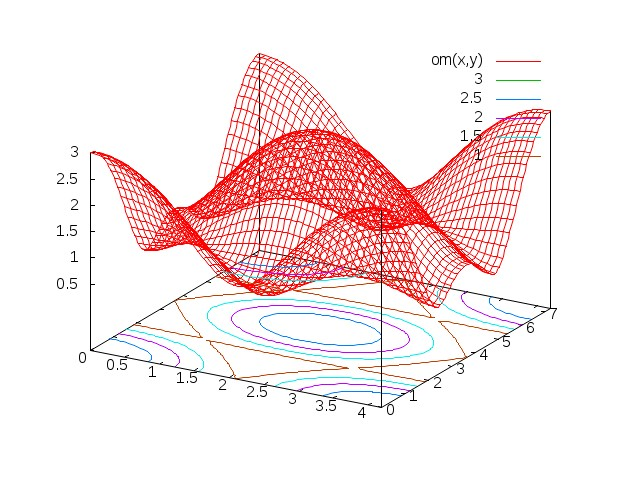
\includegraphics[width=\linewidth]{haldane_spectrum.jpg}
	\end{figure}
	\section{Полоса}
	Чтобы исследовать полосу из атомов в этой модели, нужно сделать преобразование Фурье
	только по одной координате:
	\begin{equation}
		a_{mn} = \sum \frac{e^{i\sqrt{3}p_yn}}{\sqrt{N}} a_{m,p_y}
	\end{equation}
	(и то же самое для $b$). Тогда гамильтониан запишется так:
	\begin{multline}
		H = \sum_{m, p_y} t(1+e^{-i\sqrt{3}p_ya}) a_m^\dagger b_m
		 + te^{-i\sqrt{3}p_ya} a_m^\dagger b_{m+1} + \mbox{h.c.} \\
		- 2t_2 \sin{\sqrt{3} p_ya} (a_m^\dagger a_m -  b_m^\dagger b_m)\\
		+ it_2(1 - e^{i\sqrt{3}p_ya}) (a_m^\dagger a_{m-1} - b_m^\dagger b_{m-1}) 
		+ \mbox{h.c}
	\end{multline}
	Для цепочки длиной в несколько десятков атомов собственные значения можно найти на 
	компьютере. Для $t = 1$, $t_2 = 0.3$ (данные, которые приведены в статье) уровни 
	энергии получаются такими:
	\begin{figure}[h]
		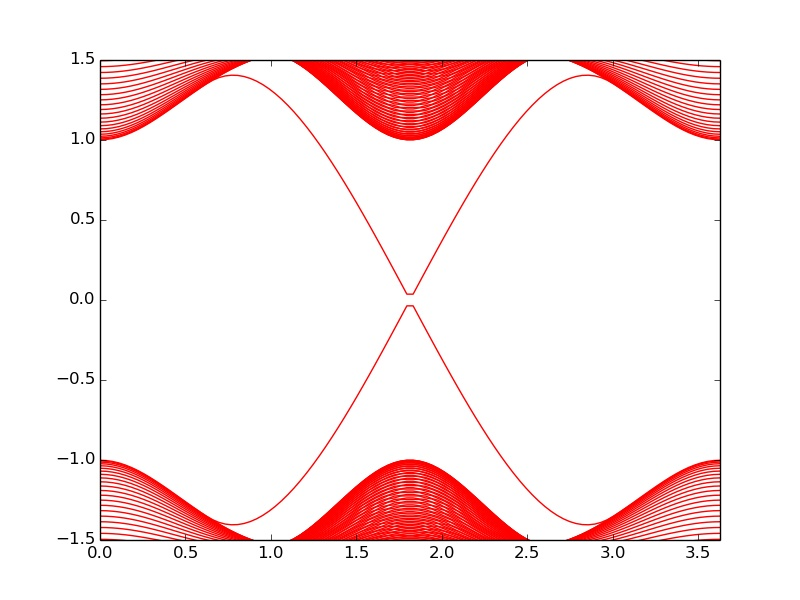
\includegraphics[width=\linewidth]{levels.jpg}
	\end{figure}

	Картинка в точности согласуется с аналогичной из статьи Кейна и Меле.
\end{document}
